\chapter{Progetto di Archivi Digitali}
\label{ch:archivi}

Questo capitolo contiene la documentazione del progetto realizzato utilizzando le tecnologie descritte nei capitoli precedenti. Si tratta di un’applicazione decentralizzata costruita attraverso la blockchain pubblica Ethereum e il protocollo IPFS. Lo scopo principale di questo progetto è la descrizione della metodologia di sviluppo in un ecosistema distribuito. Se per molti programmatori imparare un nuovo linguaggio di programmazione o framework può essere una situazione frequente, lo sviluppo in un paradigma differente richiede una descrizione più approfondita della metodologia e delle pratiche migliori da adottare durante la fase di preparazione e di sviluppo.

\section{Definizione di obiettivi e requisiti dell’applicazione}

L’obiettivo consiste nello sviluppo di un'applicazione per la registrazione di opere d’arte definibili come \emph{minori} che, potranno essere memorizzate in maniera trasparente, permanente e immutabile in una blockchain pubblica.

In dettaglio l’applicazione deve soddisfare i seguenti requisiti e funzionalità:

\begin{itemize}
\item Inserimento di oggetti nell’archivio, descritti attraverso l’utilizzo di sistemi di metadati opportuni.
\item Memorizzazione e visualizzazione degli oggetti inseriti.
\item Possibilità di modificare l’oggetto inserito da parte del suo autore mantenendo la storia completa delle modifiche effettuate.
\end{itemize}

Gli utenti previsti per l'applicazione sono di due tipi:
\begin{itemize}
\item Qualsiasi utente dotato di un indirizzo sulla rete, quindi in grado di interagire con l'applicazione, può, senza restrizioni, visualizzare tutti gli oggetti inseriti nell'archivio. Inoltre finché l'utente dispone di fondi sufficienti potrà inserire nuovi oggetti e modificare la loro descrizione.
\item Utenti dotati di permessi di verifica e approvazione dei dati inseriti nell'archivio attraverso un sistema di votazione.
\end{itemize}

Tenendo in mente questi requisiti e le considerazioni fatte nel capitolo \ref{sectionDigitalArchives}: "Blockchain negli archivi digitali" è possibile procedere con l'implementazione basata sulla blockchain Ethereum.

\subsection{Sistemi di metadati}

Prima di proseguire con la fase dello sviluppo dell'applicazione, una considerazione importante riguarda la descrizione delle risorse attraverso sistemi di metadati. Secondo una descrizione generica: “i metadati sono informazioni strutturate relative ai dati, interpretabili da parte di un computer”\footfullcite{metadatiCNR}. Inserire un oggetto dentro un archivio digitale che gestisce opere d’arte minori implica l'implementazione di un sistema di regole adatto a esprimere le diverse tipologie delle risorse in questione. Ad esempio, le risorse da rappresentare possono essere dei manoscritti, delle fotografie, dei disegni, degli oggetti di oreficeria e così via.

Esistono molti standard più o meno formali per la descrizione di particolari categorie di materiale, per questo progetto si è scelto di implementare tre modalità di rappresentazione delle risorse, le prime due appartengono allo schema di metadati Dublin Core\footfullcite{dublinCore}, mentre la terza è un esempio del modello ontologico CIDOC Conceptual Reference Model (CRM)\footfullcite{cidocCRM}.

La scelta dei metadati è stata fatta tenendo conto di diversi fattori, innanzitutto si è cercato di scegliere gli schemi in grado di rappresentare il vasto insieme di tipologie a cui possono appartenere gli oggetti dell'archivio. Inoltre, nello scenario d'uso della salvaguardia dei beni artistici, potrebbe essere importante adottare un sistema utile alle forze dell'ordine (vedi il paragrafo successivo). Infine un’altra considerazione può essere fatta relativamente alla ricerca di un compromesso tra la complessità della descrizione, la facilità di utilizzo per un utente non esperto in materia e il grado di precisione del sistema utilizzato. Per questo l’utente può scegliere tra tre modalità di inserimento, dal più semplice al più complesso. Dublin Core fornisce uno schema di meta informazioni ideato per assegnare etichette ragionevolmente interessanti per qualunque materiale digitale. È uno schema flessibile, semplice ed estendibile che si presta bene alla costruzione di form adatte per la maggior parte dei casi di utilizzo previsti.

In figura \ref{fig:progettoInserimento} è rappresentata una parte della finestra contenente il modulo di inserimento, implementato nel progetto, con le scelte relative ai sistemi di descrizione da utilizzare.

\begin{figure}[H]
\centering
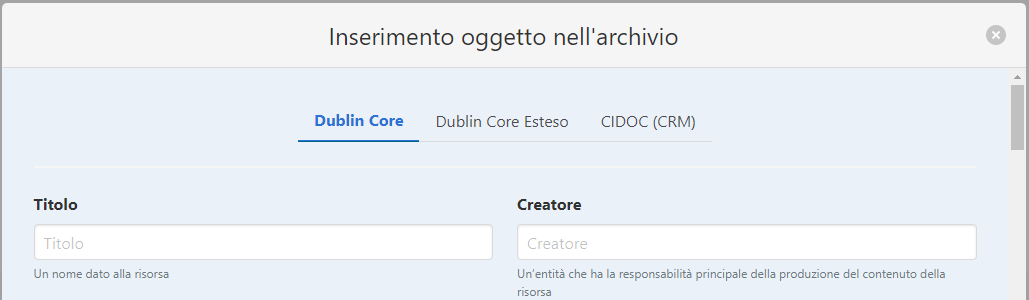
\includegraphics[width=1\textwidth]{immagini/inserimentoArchivio.PNG}
\caption{Progetto: Modulo inserimento nell'archivio}
\label{fig:progettoInserimento}
\end{figure}

La prima opzione, "Dublin Core", fornisce quindici etichette base per la descrizione delle risorse. La seconda opzione, "Dublin Core Esteso", permette una descrizione più approfondita della risorsa attraverso l'uso di qualificatori (o sottoclassi) che permettono un raffinamento dello schema con l'aggiunta di significati più precisi sui termini base. Infine la terza opzione, "CIDOC", è rivolta agli \emph{esperti} in quanto fornisce un modello ontologico formale incentrato sulla rappresentazione semantica delle risorse.

Un ultima considerazione pratica riguarda le linee guida per la descrizione di beni culturali, fornite dal nucleo carabinieri per la tutela del patrimonio culturale in figura \ref{fig:carabinieriTPC}.

\begin{figure}[H]
\centering
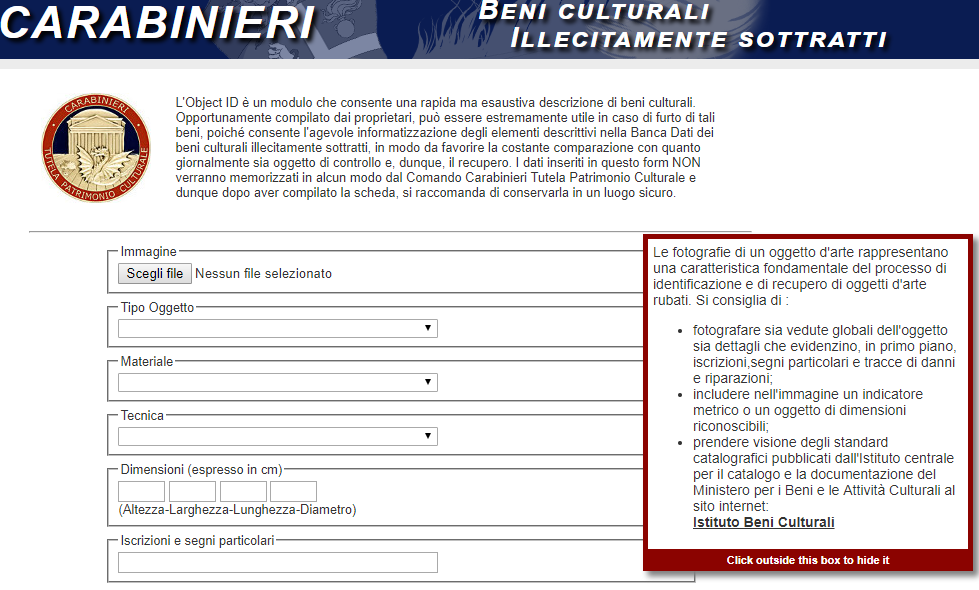
\includegraphics[width=1\textwidth]{immagini/carabinieriTPC2.png}
\caption{Beni culturali illecitamente sottratti: Modulo descrittivo}
\label{fig:carabinieriTPC}
\end{figure}

Il modulo Object ID\footfullcite{tpcCarabinieri}, adottato dalle forze dell'ordine, consente la descrizione di beni culturali ed è utile per le operazioni di recupero in caso di furto di tali beni. Quando la tecnologia sarà sufficientemente matura e testata, l'approvazione degli oggetti inseriti tramite un'applicazione basata sulla blockchain, potrebbe essere fatta dai membri autorizzati del Comando Carabinieri. Chiaramente il fatto di poter contare su una base di dati immutabile, permanente e dotata di storia completa fornirebbe dei vantaggi rilevanti rispetto ai sistemi attualmente in uso.

Con questo progetto si vuole dimostrare che è possibile adottare qualunque schema di descrizione in maniera relativamente semplice e quindi fornire una prova attendibile del possesso di tali beni. Mentre queste considerazioni sono state fatte tenendo in mente l'obiettivo consistente nella dimostrazione della metodologia, nel caso di un’applicazione pronta ad essere adottata al pubblico, questa parte assumerebbe un ruolo di primo piano per l'intero processo di sviluppo.

\section{Preparazione dell'ambiente di sviluppo}

Lo sviluppo del progetto sulla blockchain Ethereum è accompagnato dalla presenza di numerosi strumenti, in questa sezione sarà fornita la lista dei principali strumenti e delle dipendenze utilizzate durante la programmazione.

\begin{itemize}
\item NPM (Node Package Manager) per la gestione e l'installazione dei moduli/librerie Javascript. NPM richiede la presenza di Node.js\footnote{In questo progetto si è utilizzato Node.js nella versione 10.8.0 e NPM versione 6.2.0}.

\item Truffle framework (versione 4.1.14)\footfullcite{truffleFramework} un ambiente di sviluppo composto da un insieme di strumenti che facilitano la creazione delle applicazioni decentralizzate (di seguito dApps) sulla piattaforma Ethereum. Truffle gestisce il ciclo di migrazione (sulla blockchain) degli smart contracts, la loro integrazione ed esecuzione con la possibilità di eseguire test automatizzati.

Il framework include Ganache\footfullcite{ganache} (versione 1.2.2), una blockchain personale, utile per lo sviluppo locale delle dApps. Ganache è un emulatore di nodi Ethereum con un'interfaccia grafica intuitiva (in figura {\ref{fig:ganache}}), mette a disposizione un certo numero di account precaricati con Ether. Si tratta di una blockchain con un funzionamento semplificato che permette di analizzare lo stato della blockchain in qualunque momento dell'esecuzione.

\begin{figure}[H]
\centering
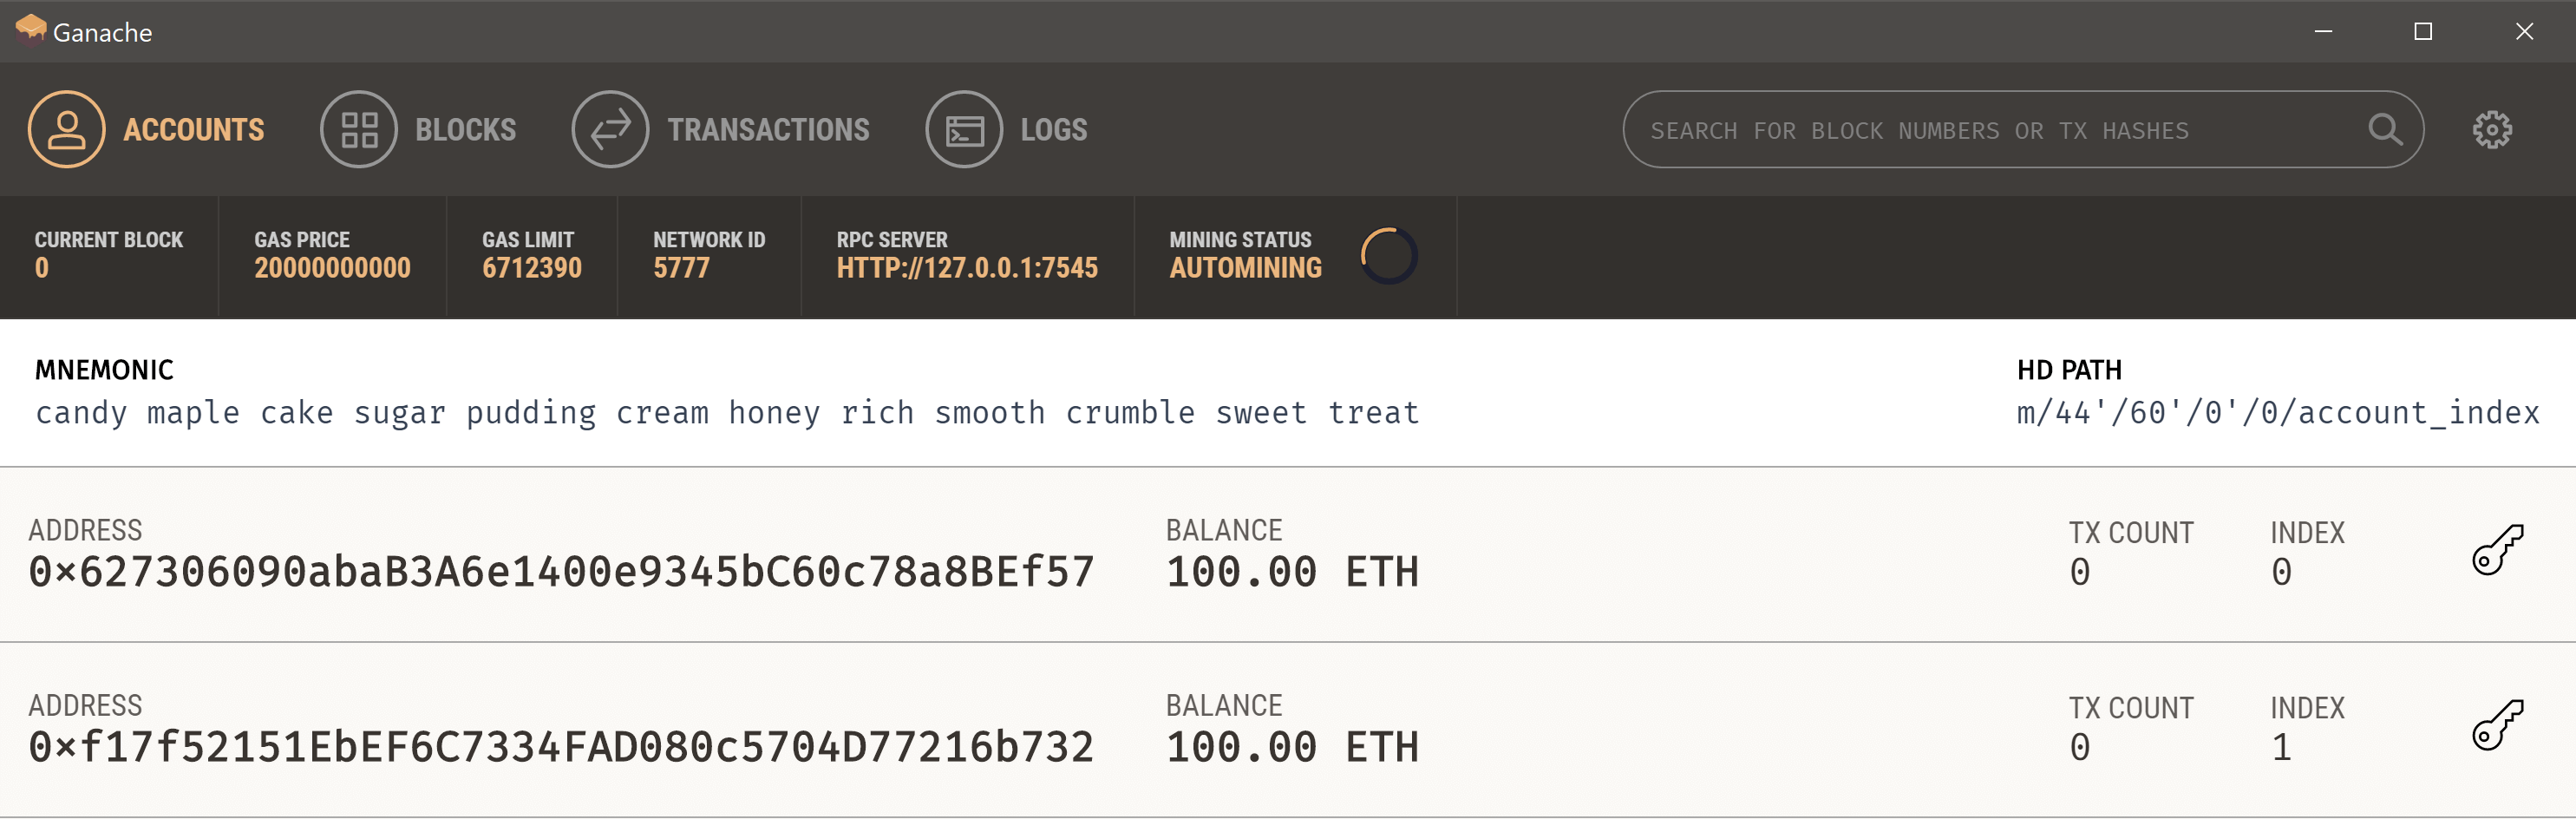
\includegraphics[width=1\textwidth]{immagini/ganache-window.png}
\caption{Ganache: Blockchain locale}
\label{fig:ganache}
\end{figure}

Truffle fornisce anche il codice \emph{boilerplate} raggruppato in diversi pacchetti chiamati "boxes", utili per uno sviluppo accelerato\footnote{Come base di questo progetto si è scelto il pacchetto chiamato pet-shop disponibile su https://truffleframework.com/boxes/pet-shop}.

\item Geth\footfullcite{geth} è l'implementazione ufficiale di un nodo completo Ethereum che permette la sincronizzazione e la partecipazione alla blockchain Ethereum.

\item Mocha e Chai sono usati per la creazione e l'esecuzione di test automatizzati. Mocha\footfullcite{mocha} è un test framework per Javascript basato su Node.js, mentre Chai\footfullcite{chai} è una libreria di asserzioni che può essere implementata sul framework. Insieme permettono l'implementazione di test automatizzati complessivi secondo un approccio TDD (Test Driven Development) e BDD (Behaviour Driven Development).

\item Metamask\footfullcite{metamask} è un’estensione, disponibile per i maggiori browser (Firefox, Chrome,Brave, ecc.). Necessario per utilizzare le dApps, fornisce un portafoglio (\emph{wallet}) che consente di identificare l'utente (attraverso la chiave pubblica) e di gestire le transazioni con la chiave privata.

\item Web3.js\footfullcite{web3} (versione 0.20) è una collezione di librerie che, attraverso un API, permette l'interazione con il codice dei contratti situati sulla blockchain. In particolare, permette di sviluppare la parte client dell'applicazione con le chiamate di lettura e di scrittura ai contratti.

\end{itemize}

Questi sono gli elementi più importanti, al momento più usati per interagire con le dApps e per sviluppare le proprie applicazioni. Altri elementi scelti per lo sviluppo di questa specifica applicazione, nella maggior parte opzionali, verranno introdotti in seguito.

\section{Sviluppo dell'applicazione}

Lo sviluppo di questo progetto può essere suddiviso in due fasi distinte:

\begin{itemize}

\item La prima fase si pone come obiettivo la creazione di un \emph{Minimal Viable Product} (MVP) cioè un prototipo che implementata le funzionalità base. Consiste principalmente nello sviluppo dei contratti, l'esecuzione di test e costruzione di un'interfaccia di prova (GUI) che permette l'interazione con i contratti in un contesto di sviluppo locale.

\item Nella seconda fase si estende l'applicazione in modo da implementare nuove funzionalità e costruire la versione finale. Questa fase consiste principalmente nell'integrazione con il servizio di storage IPFS, lo sviluppo della parte front-end finale e il trasferimento dei contratti su una blockchain Ethereum di sviluppo (\emph{testnet}).

\end{itemize}

\subsection{Scrittura dei Contratti}

Gli smart contracts scritti in Solidity costituiscono la parte back-end e contengono la logica dell'applicazione. Nel contratto principale, \emph{Archives.sol}, tra le prime operazioni si definisce la struttura degli oggetti da inserire sulla blockchain.
\\
\begin{lstlisting}[caption={Struttura degli oggetti},language=JavaScript]
struct Artwork {
    uint id; //identificatore univoco
    address author; //indirizzo dell'autore
    string name; //nome o titolo dell'oggetto
    string descriptionHash; //descrizione completa dell'oggetto
    string mainPreviewHash; //immagine rappresentativa dell'oggetto
    bool validation; //stato dell'approvazione (true o false)
    uint votesNum; //numero delle approvazioni (o voti)
}
\end{lstlisting}

Le caratteristiche degli oggetti sono definite tramite una variabile "Artwork" di tipo \emph{struct} cioè un tipo complesso definito dall'utente contenente al suo interno un insieme di proprietà che definiscono l'oggetto. Il passo successivo consiste nella costruzione di una sequenza di oggetti da memorizzare sulla blockchain. In Solidity è possibile costruire una sequenza composta da coppie chiave-valore (come in un array associativo) usando il tipo \emph{mapping}.
\\
\begin{lstlisting}[caption={Associazione chiave-valore},language=JavaScript]
mapping (uint => Artwork) public artworks;
uint artworkCounter; //contatore degli oggetti inseriti 
\end{lstlisting}

In questo modo il mapping crea una specie\footfullcite{solidityMapping} di tabella hash (inizialmente vuota\footnote{In realtà è impossibile determinare a priori la dimensione del mapping o eseguire direttamente delle iterazioni sugli elementi. Questo perché tutte le chiavi restituiranno un valore di default di tipo Artwork.}) composta da un indice univoco (uint) che si riferisce a un oggetto di tipo Artwork. Ogni volta che verrà eseguito un assegnamento di chiave-valore, il risultato sarà memorizzato sulla blockchain. Le tabelle hash sono una struttura dinamica e pertanto è necessario tenere una variabile di stato contatore in modo da tenere traccia degli oggetti effettivamente inseriti.

A questo punto analizzando il codice del contratto Archives.sol\footnote{https://github.com/lukasd2/Digital-Archives-dApp/blob/master/contracts/Archives.sol} sono state implementate le funzionalità descritte nella fase di definizione dei requisiti del progetto.
\\
\begin{lstlisting}[caption={Funzioni principali del contratto Archives.sol},language=JavaScript]
function publishArtwork(string _name, string _descriptionHash, 
                        string _dataHash) public {...}
function approveArtwork(uint _id) public onlyIfWhitelisted(
                        msg.sender) checkValidation(_id) {...}
function modifyArtworkDescription(uint _id, 
                        string _newDescriptionHash) public {...}
\end{lstlisting}

\begin{itemize}
\item La funzione "publishArtwork" gestisce l'inserimento di un nuovo oggetto nell'archivio.
\item La funzione "approveArtwork" gestisce l'approvazione degli oggetti inserti. Permette agli utenti autorizzati di votare per un dato oggetto e di controllare se il numero di voti registrati è sufficiente alla sua approvazione.
\item La funzione "modifyArtworkDescription" permette all'utente che inserisce l'oggetto di modificare la sua descrizione.
\end{itemize}

Successivamente al contratto Archives.sol sono stati aggiunti altri contratti che espandono le funzionalità e i controlli richiesti dall'applicazione. Per la costruzione della struttura dei contratti si è sfruttato il meccanismo dell'ereditarietà di Solidity, con la gerarchia rappresentata in figura \ref{fig:contractStructure}. Archives.sol si trova al livello più alto della catena e dunque può usufruire di tutte le funzioni definite nei contratti situati a livello più basso. In particolare i contratti Whitelist.sol, RBAC.sol e Roles.sol sono usati rispettivamente per aggiungere indirizzi alla lista di utenti dotati di permessi di verifica e per gestire i permessi degli utenti che acquistano lo status di "artwork checker" con i rispettivi controlli.
Il contratto Ownable.sol implementa il meccanismo di autorizzazione dell'autore del contratto, cioè all'indirizzo che pubblica il contratto sulla rete. Nella versione attuale al "proprietario" vengono dati i permessi di aggiungere nuovi utenti alla whitelist. 

\begin{figure}[H]
\centering
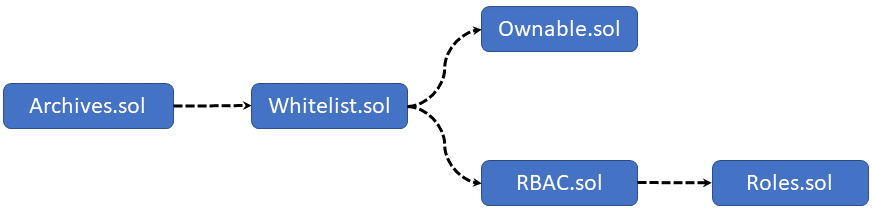
\includegraphics[width=1\textwidth]{immagini/contractStructure.png}
\caption{Progetto: Struttura dei contratti}
\label{fig:contractStructure}
\end{figure}

Questi contratti (Whitelist.sol, Ownable.sol, RBAC.sol e Roles.sol) sono stati presi dalla libreria OpenZeppelin\footfullcite{openZeppelin} contenente implementazioni delle funzionalità ricorrenti nelle dApps. Sono considerati sicuri perché ampiamente testati e aggiornati dalla comunità, questi contratti sono stati opportunamente modificati e integrati in questo progetto{\footnote{Codice di tutti i contratti implementati, https://github.com/lukasd2/Digital-Archives-dApp/tree/master/contracts}}.

\subsection{Test dei Contratti}

Una volta implementata la logica dell'applicazione è particolarmente importante assicurarsi che i contratti siano sicuri e privi di errori eseguendo dei test automatici. Gli smart contracts una volta pubblicati su Ethereum diventano immutabili, ai contratti verrà assegnato un certo indirizzo sulla blockchain e non sarà più possibile effettuare delle modifiche al loro codice a meno di caricarne altri sotto nuovi indirizzi.

Un altro aspetto importante riguarda i costi legati alla loro pubblicazione (\emph{deploy}), le nuove versioni dell'applicazione possono essere pubblicate sotto nuovi indirizzi e ogni volta sarà necessario pagare, ex novo, il prezzo (Gas) calcolato per la loro pubblicazione. Un discorso analogo può essere fatto per i costi legati alle singole transazioni del contratto, l'obiettivo ideale è quello di creare una versione dell'applicazione ottimizzata e affidabile per i casi d'uso previsti dal programma e allo stesso tempo testata per prevenire comportamenti indesiderati.

In questa applicazione i programmi di testing sono stati divisi in tre parti (DigitalArchives\_initialState.js, DigitalArchives\_events.js e DigitalArchives\_exceptions.js{\footnote{Codice dei test automatizzati, https://github.com/lukasd2/Digital-Archives-dApp/tree/master/test}}). I programmi fanno uso della libreria di asserzioni Chai, nel primo gruppo viene controllato lo stato iniziale del contratto simulando una lo stato del contratto al momento della pubblicazione sulla blockchain. Il secondo gruppo verifica l'esecuzione degli eventi e i comportamenti previsti al cambiamento dello stato in seguito alle transazioni. Infine il terzo gruppo riunisce un certo numero di scenari non permessi (\emph{edge cases}) che l'applicazione dovrebbe gestire lanciando delle eccezioni.

Di seguito nella figura \ref{fig:contractTests} è mostrata l'esecuzione di questi test con framework Truffle.
\\
\begin{lstlisting}[caption={Truffle esecuzione di test},language=JavaScript]
>> truffle test
\end{lstlisting}

\begin{figure}[H]
\centering
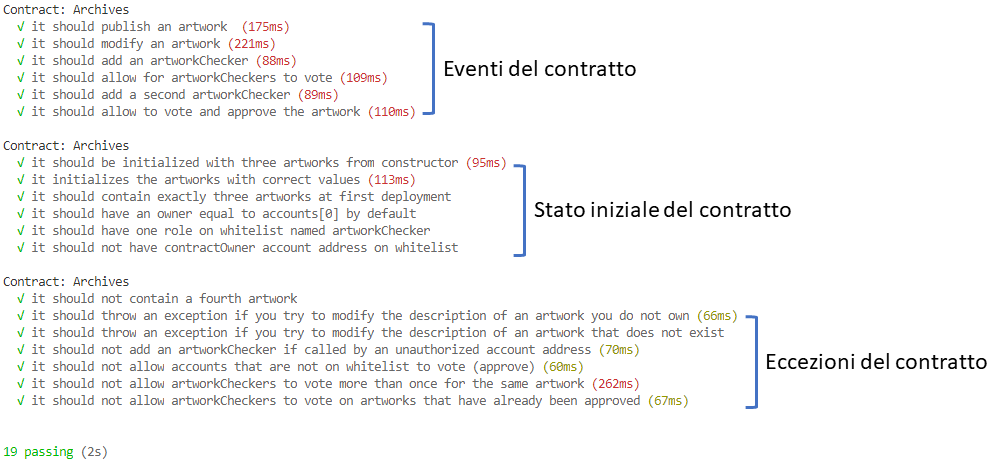
\includegraphics[width=1\textwidth]{immagini/testContratti.png}
\caption{Progetto: Risultato esecuzione dei test}
\label{fig:contractTests}
\end{figure}

\subsection{Applicazione client-side}

Ultimo passaggio della prima fase di sviluppo\footnote{Il processo di sviluppo del prototipo può essere consultato in questa repository, https://github.com/lukasd2/DigitalArchivesPrototype} consiste nella programmazione di un'interfaccia client-side da collegare con i contratti testati.

Web3.js è una collezione di librerie che permettono di effettuare operazioni di lettura e scrittura sulla blockchain, così come avviene ad esempio con \emph{Ajax} e i web server tradizionali. Fondamentalmente, a parte l’utilizzo di web3, il lato della programmazione front-end non subisce altri cambiamenti. Per le istruzioni di chiamata alla blockchain bisogna tenere conto dell’utilizzo delle funzioni asincrone e quindi gestire l’interfaccia e il flusso delle funzioni in modo adeguato per l’utente finale e per la gestione dei risultati in arrivo.

Per questo progetto si è scelto di costruire un'interfaccia minima con Bootstrap\footfullcite{bootstrap}, in figura \ref{fig:Prototipo} si vede la parte relativa all'inserimento di un oggetto nella blockchain. 

\begin{figure}[H]
\centering
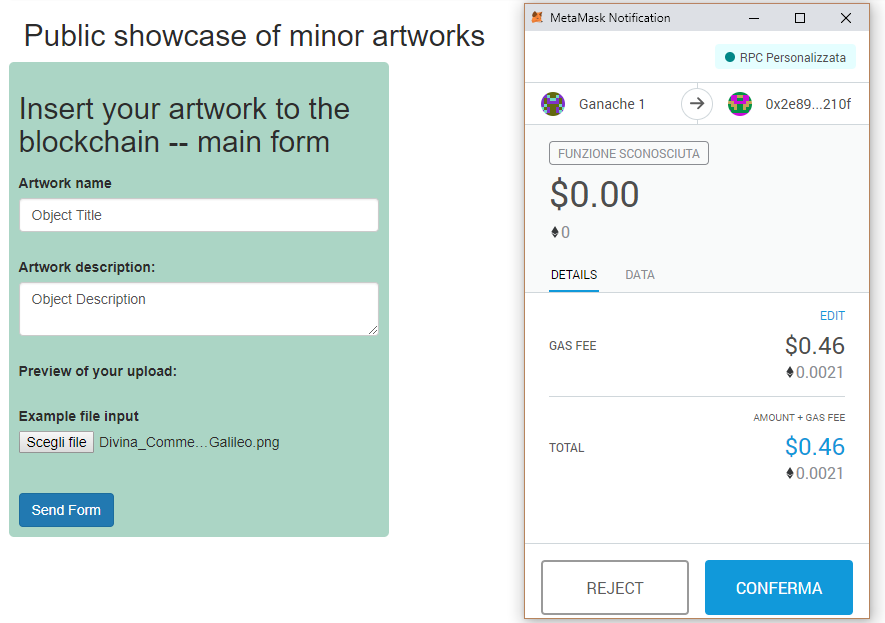
\includegraphics[width=1\textwidth]{immagini/prototype.PNG}
\caption{Progetto: Prototipazione inserimento oggetto sulla blockchain}
\label{fig:Prototipo}
\end{figure}

A questo punto è possibile testare il funzionamento della dApp attraverso l'interfaccia grafica. Per quanto riguarda le transazioni, ovvero le chiamate ai contratti che richiedono lo svolgimento di calcoli computazionali da parte della EVM, esse saranno intercettate da Metamask. In questa fase potrebbe essere utile passare da una blockchain con un funzionamento semplificato, impostando un nodo blockchain (privato) vero e proprio con Geth per accertarsi del funzionamento corretto della dApp.

\subsection{Integrazione con IPFS}

Nelle dApp che richiedono la memorizzazione di una quantità rilevante di dati, che nelle blockchain è tra le operazioni più costose, diventa indispensabile integrare un servizio di storage esterno. In questo progetto si utilizza IPFS per memorizzare e richiamare i dati troppo grandi per essere mantenuti direttamente su Ethereum. La figura \ref{fig:dapp} rappresenta l'impostazione finale della logica dell’applicazione.

\begin{figure}[H]
\centering
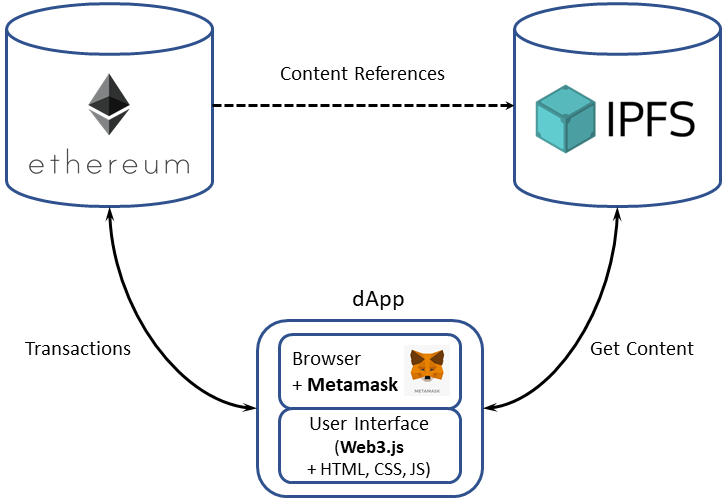
\includegraphics[width=1\textwidth]{immagini/ipfsIntegration.png}
\caption{Progetto: Logica dell'applicazione finale}
\label{fig:dapp}
\end{figure}

Seguendo questa impostazione la compilazione del modulo per l’inserimento di un nuovo oggetto include la spedizione delle risorse su IPFS. Prima di poter spedire la transazione sulla blockchain, la richiesta viene processata e rimane in attesa di upload sul servizio di storage. Se il caricamento avviene con successo, verrà restituito un indirizzo hash contenente i file caricati. A questo punto sarà possibile memorizzare il riferimento all'indirizzo IPFS sulla blockchain con una transazione. Ricapitolando, l'oggetto, la cui struttura è definita nel contratto, conterrà un puntatore all'indirizzo IPFS contenente la sua descrizione.
\\
\begin{lstlisting}[caption={Riferimento all'indirizzo hash di IPFS},language=JavaScript]
struct Artwork {
    ...
    string descriptionHash; //hash della descrizione dell'oggetto 
}
\end{lstlisting}

In questo modo si sfrutta la caratteristica di IPFS dell'indirizzamento basato sul contenuto, per cui è matematicamente certo che sotto un indirizzo hash sarà possibile trovare un dato dal contenuto immutabile, e con il progredire della tecnologia, permanente. Riguardo alla permanenza, il sistema IPFS allo stato dell'arte non ha implementato un meccanismo di incentivi, per cui, in questa applicazione, la memorizzazione viene effettuata attraverso Infura\footfullcite{infura}, una API che agisce da intermediario, in modo da mantenere il contenuto accessibile senza bisogno di mantenere un nodo personale (IPFS) costantemente attivo. Dunque una chiamata generica di caricamento del contenuto su IPFS avrà la seguente struttura:
\\
\begin{lstlisting}[caption={Aggiunta di file con IPFS Javascript API},language=JavaScript]
ipfs.files.add(data, [options], [callback])
\end{lstlisting}

Una delle principali funzionalità dell'applicazione, l'inserimento dell'oggetto sulla blockchain, è composta dalla seguente catena di operazioni:

\begin{enumerate}
    \item L'utente compila il modulo descrittivo dell'oggetto e preme il pulsante "Inserisci Oggetto"
    \item Il programma cattura i file (in questa implementazione immagini) rappresentative dell'oggetto e attraverso un Buffer\footnote{https://www.npmjs.com/package/buffer} li trasforma in una sequenza di dati binari
    \item La sequenza di bit viene caricata su IPFS
    \item IPFS ritorna un indirizzo hash per ciascuno dei file caricati che vengono memorizzati nella sessione in esecuzione del programma
    \item Il programma costruisce una descrizione completa dell'oggetto utilizzando la versione del sistema di metadati scelta dall'utente e include gli indirizzi hash dei file caricati. Con un’altra operazione di caricamento su IPFS il tutto viene raggruppato sotto un unico indirizzo hash che viene restituito al programma in esecuzione
    \item Il riferimento hash adesso può essere spedito e memorizzato sulla blockchain con una transazione effettuata e confermata dall'utente attraverso Metamask
    \item La descrizione completa dell'oggetto viene richiamata utilizzando il riferimento memorizzato sulla blockchain che punta alla posizione contenuta su IPFS
\end{enumerate}


\subsection{Costruzione dell'interfaccia finale}

Una volta implementata la logica completa dell’applicazione, seguita da una fase di test per verificarne la correttezza, è stata costruita l’interfaccia grafica finale. Per questa fase di programmazione \emph{front-end} si è scelto di utilizzare Bulma\footfullcite{bulma} e Sass\footfullcite{sass}. Bulma è un framework CSS basato su \emph{flexbox} con un certo numero di elementi grafici predefiniti e un sistema di griglia che facilita la costruzione di layout flessibili, mentre Sass è un preprocessore CSS, serve principalmente per velocizzare e rendere più efficiente lo sviluppo dei fogli di stile\footnote{Sass estende i fogli di stile con diverse funzionalità tra cui la possibilità di utilizzare variabili, funzioni modulari (mixins), operazioni matematiche ecc.}. In figura \ref{fig:indexApp} è possibile vedere la pagina iniziale dell'applicazione.

\begin{figure}[H]
\centering
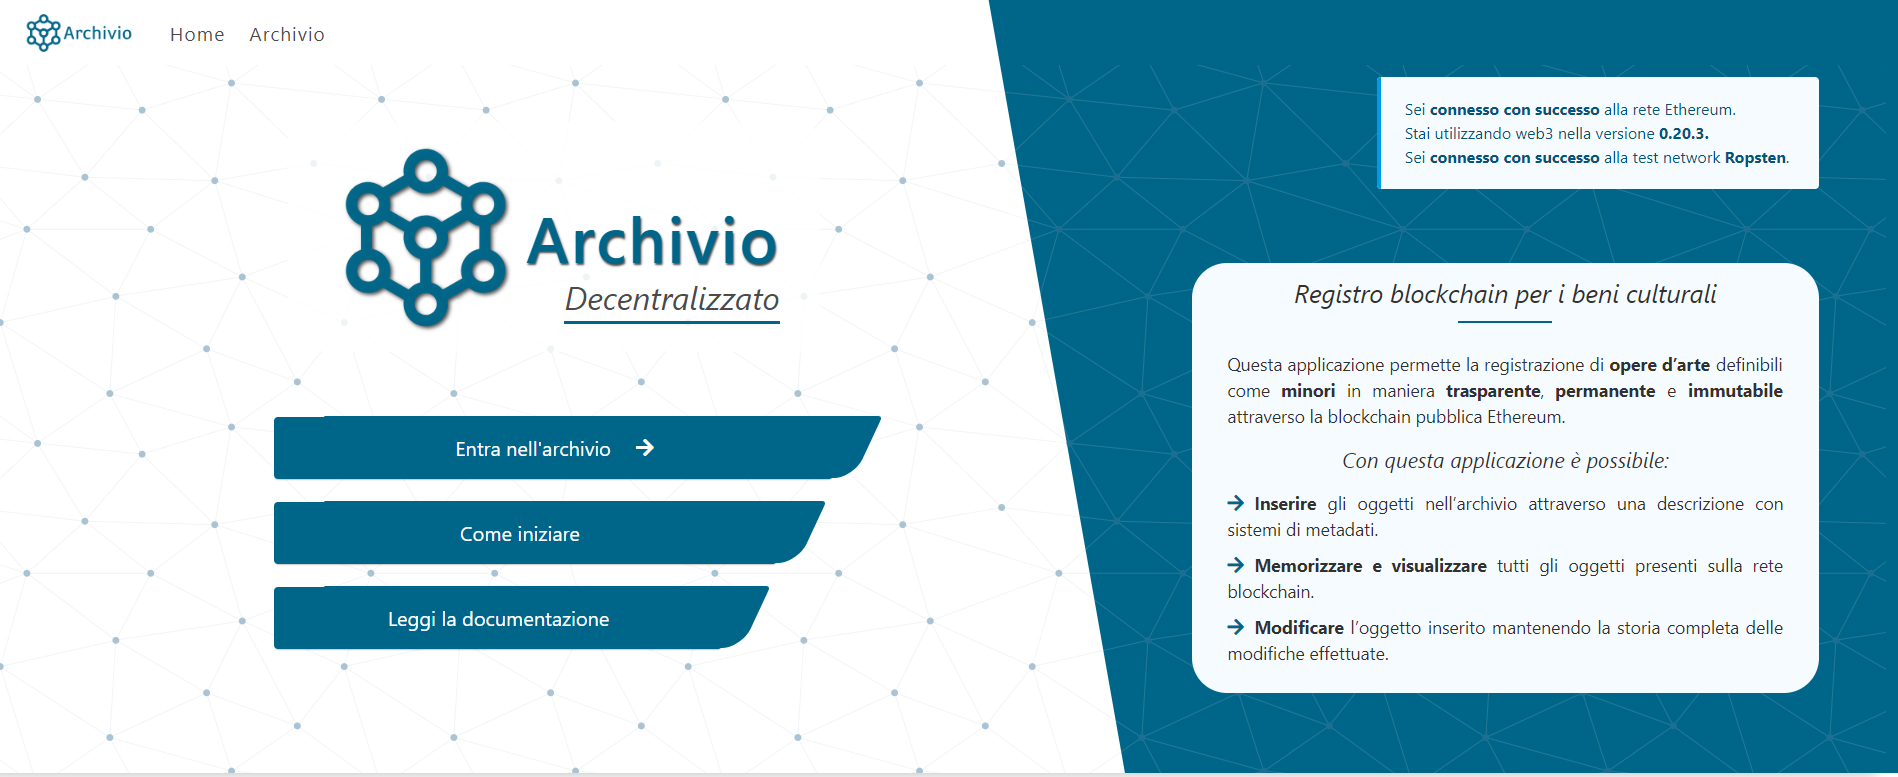
\includegraphics[width=1\textwidth]{immagini/prova3Index.PNG}
\caption{Progetto: Pagina iniziale dell'applicazione}
\label{fig:indexApp}
\end{figure}

Questa pagina serve a dare informazioni essenziali sulle funzionalità del progetto e i vantaggi derivanti dall'utilizzo della blockchain. Inoltre serve da guida per l'utilizzo delle dApps e si ricollega direttamente ai contenuti di questo elaborato.

La parte principale dell'applicazione, contente l'archivio, è illustrata in figura \ref{fig:artworkApp}.

\begin{figure}[H]
\centering
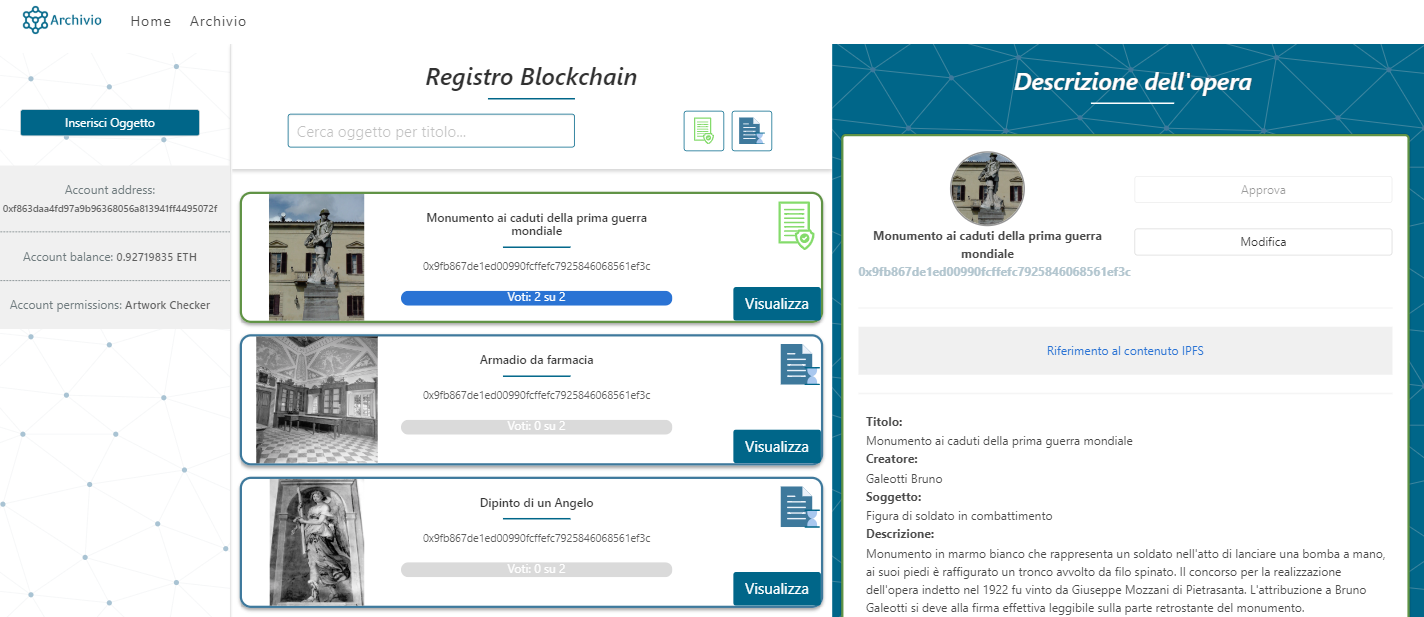
\includegraphics[width=1\textwidth]{immagini/artwork3Prova.PNG}
\caption{Progetto: Pagina contente l'archivio blockchain}
\label{fig:artworkApp}
\end{figure}

Con questa impostazione dell'interfaccia finale l'applicazione è divisa logicamente, da sinistra verso destra, in tre parti. Nella parte sinistra è possibile attivare il modulo per l'inserimento di un oggetto nel registro e consultare le informazioni principali relative al proprio account (l'indirizzo utente, il bilancio di token e i permessi). 

La parte centrale contiene l'archivio di tutte le opere registrate sulla blockchain e le informazioni principali relative a ciascun oggetto come illustrato di seguito nella figura \ref{fig:artworkFocus}. Inoltre permette di "filtrare" gli oggetti in base al loro stato di approvazione e di effettuare una ricerca per titolo tramite un input situato in alto a sinistra.

La parte a destra contiene la descrizione completa di ciascun oggetto inserito nell'archivio. In particolare i metadati e le immagini descrittive vengono richiamate da IPFS attraverso l'indirizzo hash memorizzato direttamente sulla blockchain. Una volta selezionato l'oggetto dell'archivio tramite il pulsante "visualizza", queste informazioni saranno raggruppate e compariranno in questa sezione del sito. 

\begin{figure}[H]
\centering
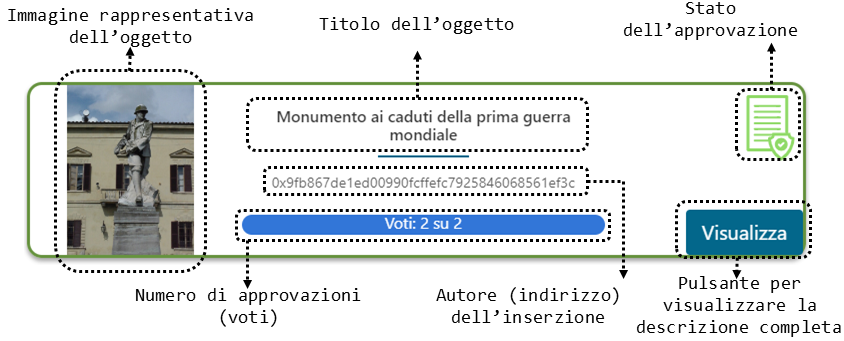
\includegraphics[width=1\textwidth]{immagini/artworkFocusCommented.png}
\caption{Progetto: Archivio la scheda di un oggetto}
\label{fig:artworkFocus}
\end{figure}

\subsection{Ethereum Testnet}

Il trasferimento dei contratti su una blockchain Ethereum di prova (\emph{testnet}) conclude lo sviluppo di questo progetto. Ethereum ha diverse reti di sviluppo, comunemente chiamate testnet, utili allo scopo di provare il funzionamento dei contratti prima di farne il deploy sulla rete principale. 

La differenza fondamentale tra queste reti e la rete principale (\emph{mainnet}) deriva dall’utilizzo di token che non hanno un valore reale al di fuori dell'ambiente di prova, dunque è possibile creare le proprie applicazioni e pubblicarle eseguendo dei test sulla determinata blockchain di sviluppo evitando di dover sostenere spese legate alle transazioni.

In questo progetto si è scelto di pubblicare i contratti su Ropsten\footfullcite{ropsten}, una blockchain di prova che, al momento dello scrivere, utilizza lo stesso sistema di consenso (Proof of Work) della rete principale. È una rete in grado di riprodurre con un buon grado di precisione il funzionamento di mainnet, questo è particolarmente utile per verificare le stime relative ai costi delle transazioni e tutti gli aspetti legati al funzionamento della dApp stessa. Questa fase risulta fondamentale nel processo di sviluppo di un’applicazione decentralizzata ed è raccomandabile effettuarla con un numero di utenti il più ampio possibile per raccogliere i dati (\emph{feedback}) circa il funzionamento di smart contracts e delle dApps in modo da trovare eventuali errori prima di pubblicare l'applicazione sulla blockchain principale.